\documentclass[twoside,a4paper,openright,titlepage,draft]{ctexrep}
\usepackage[final]{graphicx}
\usepackage{subfig}
% \usepackage{subcaption}
\usepackage{extarrows}
\usepackage{multicol}
\usepackage{float}
\usepackage{amsmath}
\usepackage{subfig}
\usepackage{cancel}
\usepackage{wrapfig}
\graphicspath{{./pictures}}
\setcounter{secnumdepth}{3}

\begin{document}
\section{Cascode放大器}
\subsection{共源共栅极放大电路}
\begin{multicols}{2}
    \begin{figure}[H]
        \centering
        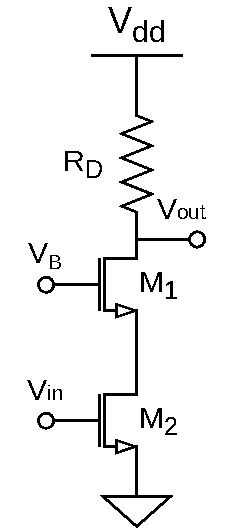
\includegraphics[height=60mm]{commonsourcegate.drawio.pdf}
        \caption{共源共栅极放大电路}
        \label{fig:共源共栅极放大电路}
    \end{figure}
    \columnbreak
    \subsubsection{Large Signal Behavior:}
    \begin{itemize}
        \item Input:
        \begin{itemize}
            \item[] $V_{in} > V_{th1}$
        \end{itemize}
        \item Output:
        \begin{itemize}
            \item[] $V_{x} > V_{gs1} - V_{th2}$
            \item[] $V_b > V_x + V_{th2}$
            \item[] $V_{out} - V_x > V_{gs2} - V_{th2}$
        \end{itemize}
        \item So:
        \begin{itemize}
            \item[] $V_{out} > V_{gs1} - V_{th1} + (V_{gs2} - V_{th2})$
        \end{itemize}
    \end{itemize}
\end{multicols}
为了使$V_{out}$的swing尽可能大,要使$V_b$尽可能低。
最低值就是:
\begin{equation}
    V_b = V_x + V_{gs2} > V_x + V_{th2} > V_{gs1} - V_{th1} + V_{th2}
\end{equation}
\subsection{小信号增益Gain}
\begin{figure}[H]
    \centering
    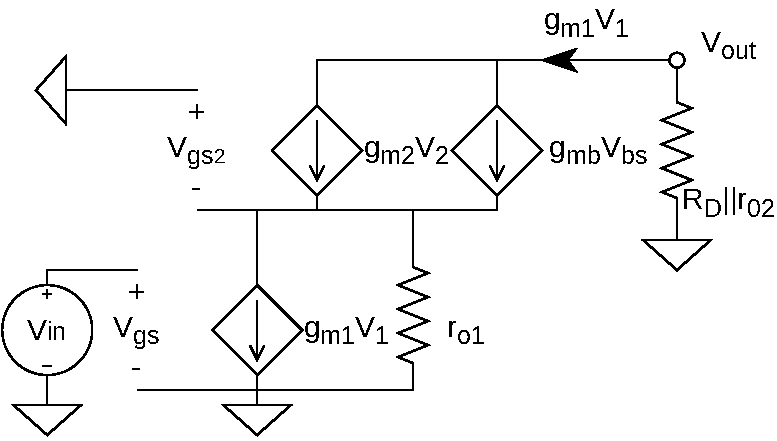
\includegraphics[width=0.6\textwidth]{smallsignal.drawio.pdf}
    \caption{Cascode小信号模型图}
    \label{fig:小信号模型图}
\end{figure}
\begin{align}
    A_V &= G_mr_{out} \notag \\
    &= -g_{m1}r_{o1}[(g_{m2} + g_{mb2})r_{o2} + 1]\notag \\
    &= A_{V1}\times A_{V2}
\end{align}
\subsubsection{输出电阻}
\begin{multicols}{2}
    \begin{figure}[H]
        \centering
        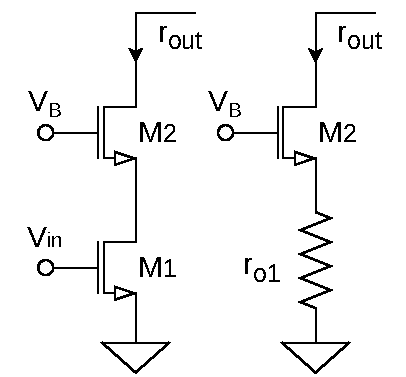
\includegraphics[height=40mm]{outputimpedence.drawio.pdf}
        \caption{测量小信号输出电阻}
        \label{fig:测量小信号输出电阻}
    \end{figure}
    \columnbreak
    \begin{align}
        r_{out} &= r_{o1} + r_{o2} + (g_{m1} + g_{m2})r_{o1}r_{o2} \notag \\
        &\approx [r_{o1}r_{o2}(g_{m1} + g_{m2})]
    \end{align}    
\end{multicols}
\subsubsection{Transconductance$G_m$}
\begin{align}
    G_m = -\frac{g_{m1}r_{o1}[r_{o2}(g_{m2}+g_{mb2})+1]}{r_{o1}r_{o2}(g_{m2}+g_{mb2})+r_{o1}+r_{o2}}
\end{align}
\subsection{Triple Cascode放大器}
\begin{multicols}{2}
    \begin{figure}[H]
        \centering
        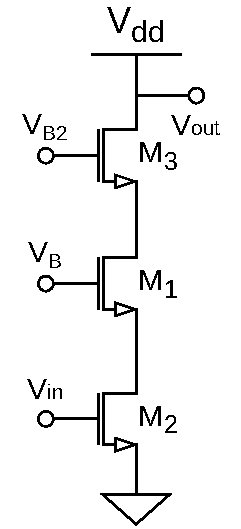
\includegraphics[height=60mm]{triplecascode.drawio.pdf}
        \caption{Triple Cascode放大器}
        \label{fig:Triple Cascode放大器}
    \end{figure}
    \columnbreak
    \subsubsection{小信号增益Gain}
    \begin{align}
        A_V = &g_{m1}r_{o1} \notag \\
        &[r_{o2}(g_{m2}+g_{mb2})+1] \notag \\
        &[r_{o3}(g_{m3}+g_{mb3})+1]
    \end{align}    
\end{multicols}
\subsubsection{输出电阻}
\begin{align}
    r_{out} = (g_{m3} + g_{mb3})\{[1+(g_{m2}+g_{mb2})r_{o2}]r_{o1}+r_{o2}\}r_{o3}+r_{o3}
\end{align}
\subsection{另一种Cascode放大器}
\begin{multicols}{2}
    \begin{figure}[H]
        \centering
        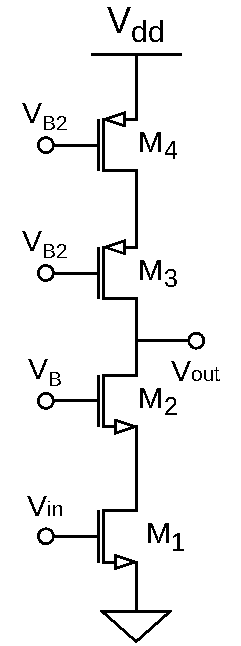
\includegraphics[height=75mm]{another.drawio.pdf}
        \caption{另一种Cascode共源共栅放大器}
        \label{fig:another}
    \end{figure}
    \columnbreak
    \subsubsection{Gain}
    \begin{align}
        A_V&=\notag \\
        &= g_{m1}[(g_{m2}r_{o1}r_{o2})\notag \\
            &\ \ \ \ ||\ (g_{m3}r_{o4}r_{o3})]
    \end{align}
    \subsubsection{$r_{out}$}
    \begin{align}
        r_{out}&= (r_{o1}+r_{o2}+r_{o1}r_{o2}(g_{m2}+g_{mb2})) \notag \\
        &||(r_{o3}+r_{o4}+r_{o3}r_{o4}(g_{m3}+g_{mb3})) \notag
    \end{align}
    这个电路有一个问题:Output Swing特别小,为($V_{dd} - 4\ \times$过驱动电压)。
\end{multicols}
\subsection{Folded-Cascode放大器}
\begin{multicols}{2}
    \begin{figure}[H]
        \centering
        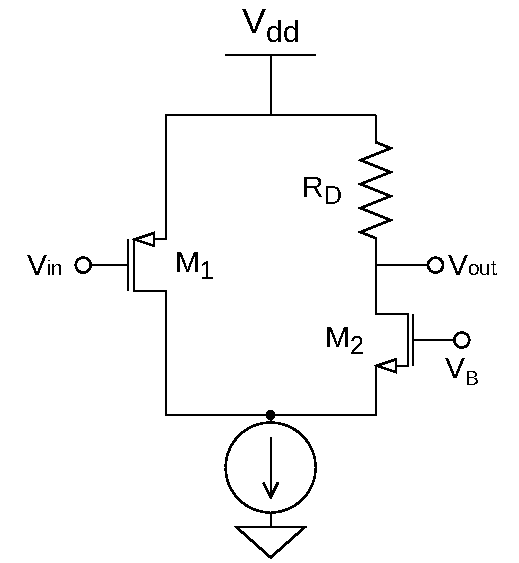
\includegraphics[height=50mm]{foldedcascode.drawio.pdf}
        \caption{Folded-Cascode放大器}
        \label{fig:foldedcascode}
    \end{figure}
    \columnbreak
    \begin{figure}[H]
        \centering
        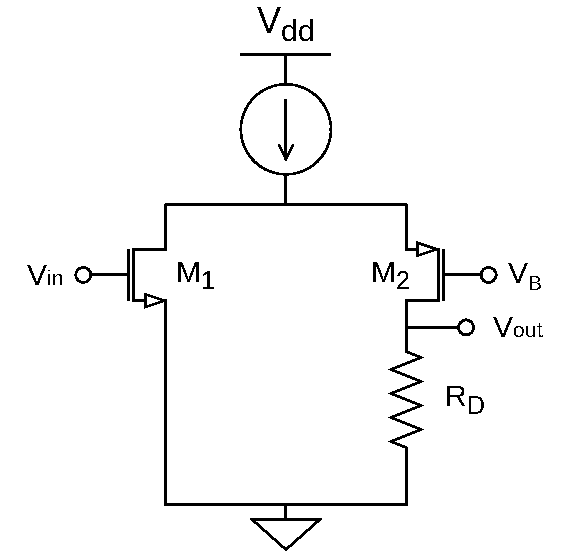
\includegraphics[height=50mm]{foldedcascode2.drawio.pdf}
        \caption{Folded-Cascode放大器}
        \label{fig:foldedcascode}
    \end{figure}
\end{multicols}
\subsubsection{大信号特性}
\begin{itemize}
    \item $V_{in}>V_{DD}-|V_{TH1}|$,$M_1$关断,$M_2$承载了所有电流$I_1$
    \item $V_{in}<V_{DD}-|V_{TH1}|$,$M_1$开启并工作在饱和区
    \item $V_{in}$继续降低,到达$I_{D1}=I_1$的时候,$M_2$关断,此时$V_{in}=V_{in1}$
    \item 当$V_{in}$继续降低,$V_{in}<V_{in1}$的时候,$M_1$进入三极管区
\end{itemize}
\subsubsection{小信号分析}

\end{document}